\documentclass{article}

\usepackage{here}
\usepackage{float}
\usepackage{adjustbox}
\usepackage{graphicx}
\usepackage{cite}
\usepackage{amsmath}
\usepackage{amssymb}
\usepackage{pifont}
\usepackage{enumitem}
\usepackage{url}
\usepackage{multirow}
\usepackage{etoolbox}
\usepackage{titlesec}
\newcommand{\cmark}{\ding{51}}

\DeclareMathOperator\erf{erf}

\interdisplaylinepenalty=2500
\hyphenation{op-tical net-works semi-conduc-tor}
\patchcmd{\thebibliography}{\section*{\refname}}{}{}{}
\setcounter{secnumdepth}{4}
\titleformat{\paragraph}
{\normalfont\normalsize\bfseries}{\theparagraph}{1em}{}
\titlespacing*{\paragraph}
{0pt}{3.25ex plus 1ex minus .2ex}{1.5ex plus .2ex}


\begin{document}

\title{The potential of a large dust grain in a collisionless plasma}
\author{Dogan Akpinar and George E. B. Doran}
\markboth{D. Akpinar \& G. E. B. Doran}
{Shell \MakeLowercase{\textit{et al.}}:}

\maketitle

\begin{abstract}
Abstract goes here
\end{abstract}

\section{Introduction}

\section{Radial motion theory (ABR)}

\smallskip

The ABR model is a radial motion theory derived by Allen, Boyd and Reynolds. It describes the equilibrium surface potential acquired
by a dust grain immersed in an infinite and stationary plasma \cite{ABR}.

\medskip

Consider a spherical dust grain, of arbitrary radius $a$, immersed in this infinite plasma. Far from the surface we assume that the electron
and ion densities are equal, denoted $n_e$ and $n_i$ respectively; this is known as quasi-neutrality, which is mathematically written as
$Zn_i \approx n_e$. As electrons are faster than ions, it can be shown that such a dust grain will become negatively 
charged \cite{Thomas}, thus ions will experience an attractive force due to the potential on the dust surface, 
$\phi_a$. We assume that ions at infinity have no kinetic energy, hence, they move radially
towards the dust grain. Therefore, it is appropriate to say that an ion at a distance 
$r$ from the dust center has radial speed $v_i$. Using energy conservation, one can show the following,

\begin{equation}\label{eq:EnergyConservation}
\frac{1}{2} m_i v_i^2 = -Ze\phi(r),
\end{equation}

\noindent where $m_i$ is the ion mass, $Z$ is the relative ion charge, $e$ is the electron charge and
$\phi(r)$ is the potential at $r$, which vanishes as $r \to \infty$ \cite{ABR}.

\medskip

Equation (\ref{eq:EnergyConservation}) then leads to an expression for the ion current, which is entirely dependant on the radial distance from the 
dust grain, given by

\begin{equation}\label{eq:ABRIi}
I_i = \frac{4\sqrt{2} \ n_i \pi r^2 Z^{\frac{3}{2}}e^{\frac{3}{2}} \phi_a^{\frac{1}{2}} } {m_i^{\frac{1}{2}}}.
\end{equation}

As the potential is negative, few electrons reach the dust grain, hence, the electron density obeys a Boltzmann
distribution:

\begin{equation}\label{eq:ABRed}
n_e(r) = n_0 \exp{\left(\frac{e\phi_a}{k_B T_e}\right)},
\end{equation}

\noindent where $n_0$ is the electron density at infinity, $k_B$ is the Boltzmann constant and $T_e$ is the electron temperature.
We further assume that only inbound electrons contribute to the electron current at the surface of the dust
grain, given as

\begin{equation}\label{eq:ABRIe}
I_i = I_e = 4 \pi a^2 n_0 e \sqrt{\frac{k_B T_e}{2 \pi m_e }} \exp{\left(\frac{e \phi_a}{k_B T_e}\right)}.
\end{equation}  

\noindent where $m_e$ is the electron mass \cite{ABR}.

\medskip

It is useful to apply the following normalisations, noting that $\Phi$ is the opposite
sign for simplicity:

\begin{equation}\label{eq:ABRnorm}
{\Phi = - \frac{e\phi}{k_B T_e}}, \ {\rho = \frac{r}{\lambda_D}},\ {\alpha = \frac{a}{\lambda_D}},\ {J = \frac{I_i}{4 \pi \lambda_D^2 n_0 e \sqrt{\frac{2k_B T_e}{m_i}}}},
\end{equation}
    
\noindent where $\lambda_D$ is the electron Debye length, which is 
a characteristic length over which quasi-neutrality breaks down,

\begin{equation}\label{eq:Debye}
\lambda_D = \sqrt{\frac{\varepsilon_{0} k_{B} T_{e}}{n_{0} e^2}}.
\end{equation}

\smallskip

Poisson's law allows for the formation of a differential equation which relates
the spatial variation of the potential to the difference in electron and 
ion densities,

\begin{equation}\label{eq:ABR9} 
\frac{d}{d\rho} \left(\rho^2 \frac{d\Phi}{d\rho}\right) = J Z^{-\frac{1}{2}}\Phi^{-\frac{1}{2}}  - \rho^2 \exp{(-\Phi)}.
\end{equation}

\smallskip

\noindent This equation may be solved using the boundary conditions;

\begin{equation}\label{eq:ABR10}
\rho \approx J^{\frac{1}{2}} Z^{-\frac{1}{4}} \Phi^{-\frac{1}{4}} \exp{\left(\frac{\Phi}{2}\right)},
\end{equation}
 
\begin{equation}\label{eq:ABR11}
\frac{d\Phi}{d\rho}\biggr|_{\rho_b} = \frac{2\rho_b Z^{\frac{1}{2}} J^{-1} \Phi_b^{\frac{3}{2}}}{\Phi_b - \frac{1}{2}} exp{(-\Phi_b)},
\end{equation}
 
\begin{equation}\label{eq:ABR13}
\frac{J}{\Gamma} = \frac{4Z^{\frac{1}{2}}\Phi_b^{\frac{3}{2}}(2\Phi_b - 3)(2\Phi_b + 1)}{(2\Phi_b - 1)^3},
\end{equation}

\begin{equation}\label{eq:ABR12}
\frac{J}{\alpha^2} = \frac{\mu}{\sqrt{4\pi}} \exp{\left(-\Phi_a\right)},
\end{equation}

\smallskip

\noindent which are formed by assuming that there exists a certain distance $\rho_b$, past which, quasi-neutrality applies. 
The potential at $\rho_b$ is given by $\Phi_b$ and $\Gamma$ is a number much greater than unity \cite{ABR}.
In order to find a value for the surface potential we must solve (\ref{eq:ABR9}), this may be 
achieved using a 4th order Runge-Kutta. We choose $\Gamma = 10000$ and find the roots of 
(\ref{eq:ABR13}) allowing us to determine the necessary boundary conditions 
using (\ref{eq:ABR10}) and (\ref{eq:ABR11}). Hence, solving the differential equation numerically yields 
the following graph of normalised dust potential as a function of normalised dust radius.

\begin{figure}[H]
\centering
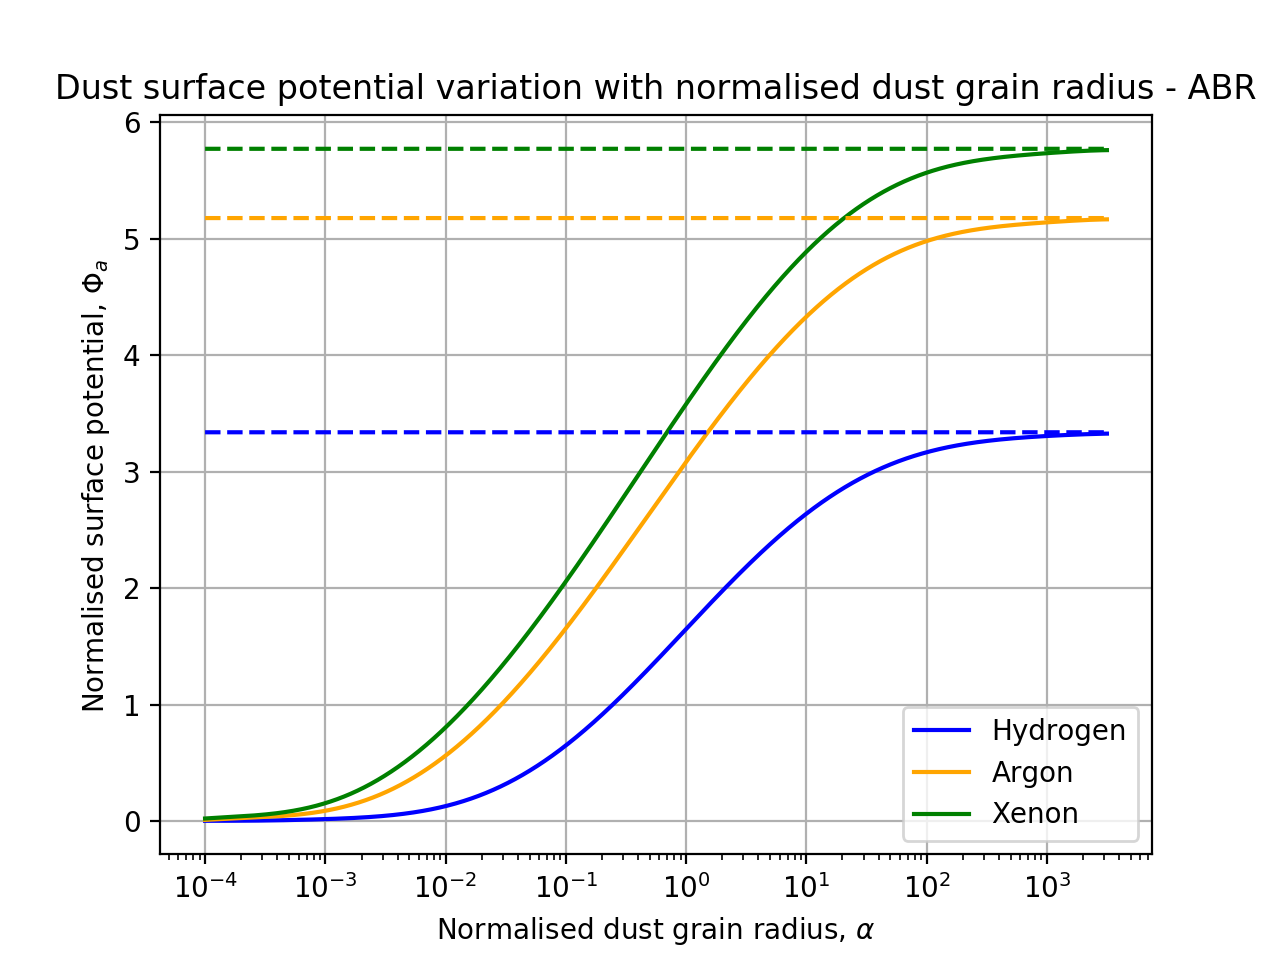
\includegraphics[width=\linewidth]{Output/ABRgraph.jpeg}
\caption{ABR predictions for $\Phi_a$ as a function of $\alpha$ for a dust grain in singly ionised Hydrogen, Argon and Xenon plasmas ($Z=1$) \cite{ABR} \cite{Thomas}.}
\label{ABR} 
\end{figure}

Thomas \cite{Thomas} discusses that in the limit of $\alpha \to \infty$ the ABR potential approaches
the cold planar wall limit, given as the following 

\begin{equation}\label{eq:ABRLim}
\lim_{\alpha \to \infty} \Phi_a = \frac{1}{2}\ln{\left(2 \pi \right)} - \frac{1}{2} - \ln{\left(\mu \right)},
\end{equation}

\noindent where the $-\frac{1}{2}$ is due to the potential drop across a cold ion pre-sheath, $\Theta = 0$,
as discussed by Stangeby \cite{Stangeby1986}. Furthermore, one can clearly see that in the limit
of $\alpha \to 0$ the ABR prediction tends to zero also, which makes physical sense \cite{ABR}.



\section{Modified orbital motion limited (MOML)}
\section{SCEPTIC numerical fit}
\section{Comparison of MOML and ABR with SCEPTIC data}
\section{Flowing sheath approximation}
\section{Conclusion}


\section{References and Acknowledgements}
\bibliography{DustyLib}
\bibliographystyle{IEEEtran}

\section{Appendix}

\subsection{Symbol dictionary}
\begin{center}
\begin{tabular}{cl} 

$e$ & Electron charge \\
$\varepsilon_0$ & Permittivity of free space \\
$k_B$ & Boltzmann's constant \\
$a$ & Dust radius\\
$\alpha$ & Normalised dust radius \\
$_a$ & Subscript indicating a quantity at the dust grain surface \\
$r$ & Distance from the centre of the dust grain \\
$\rho$ & Normalised distance from the centre of the dust grain \\
$\lambda_D$ & Debye length \\
$m_j$ & Mass \\
$n_j$ & Density \\
$T_j$ & Temperature \\
$I_j$ & Current \\
$_j$ & Subscript indicating a plasma particle \\
$_i$ & Subscript indicating an ion quantity \\
$_e$ & Subscript indicating an electron quantity \\
$_0$ & Subscript indicating an electron quantity at infinity \\
$\mu$ & Root mass ratio\\
$\Theta$ & Ratio of ion to electron temperature \\
$\gamma$ & Heat capacity ratio \\
$u$ & Flow velocity \\
$\upsilon$ & Normalised flow velocity \\
$\Gamma$ & ABR correction factor \\
$Z$ & Ion charge number \\
$Q$ & Dust grain charge \\
$\phi$ & Electric potential \\
$\Phi$ & Normalised electric potential \\

\end{tabular}
\end{center}



\end{document}